% !TEX root = ./../../_Thesis.tex

% section's Name and Label
\section{Measurements}
\label{sec:Apparatus_and_Measurements}

We have designed an auxiliary apparatus to estimate the absolute threshold for vision. The device, built using a 3-D printer, consists of a tube with one of its ends containing a support for lenses and the fixation of an eyecup, while the other end holds a smartphone (Figure~\ref{fig:3d_apparatus}).    
The eyecup end holds an 8.0 D plano-convex lens, making the length of the tube equal to this lens focal distance (12.5 cm). With such configuration, the light coming from a pixel from the smartphone's screen reaches the subject's eye as a set of parallel rays. Thus,  this is equivalent to observing a point at infinity. 
% and the mobile device's screen was set to 12.5 cm, aiming parallel rays when looking at the screen. Further,
The eyecup was adapted from a viewfinder of the DSLR camera. The device was completely painted with a dull black paint to avoid reflections in its interior. 
% used in the optical experiments.
%
%to isolate external light and place lens. Many trial versions of it are illustrated in Figure~\ref{fig:older_prot}, while the final one, built in a 3-D printer, is shown in Figure~\ref{fig:new_prot}. 
For the experiments, we have used an iPhone 5 to generate light stimulus and control its intensity. The iPhone 5 uses a Retina Display
($1,136 \times 640$ pixels) with 326 pixels per inch. 
%The distance between the plano-convex lens (8 diopters) and the mobile device's screen was set to 12.5 cm, aiming parallel rays when looking at the screen. Further, the eyecup was adapted from the viewfinder of the DSLR camera used in the optical experiments. 
%Figure~\ref{fig:slice} shows the interior of the apparatus, which has two other distances besides the focal length (12.5 cm). But just the middle one (\ie, the focal length) was explored during the experiments. 
%
\begin{figure}[!t]
	\centering
	
	\subfigure[]{
%		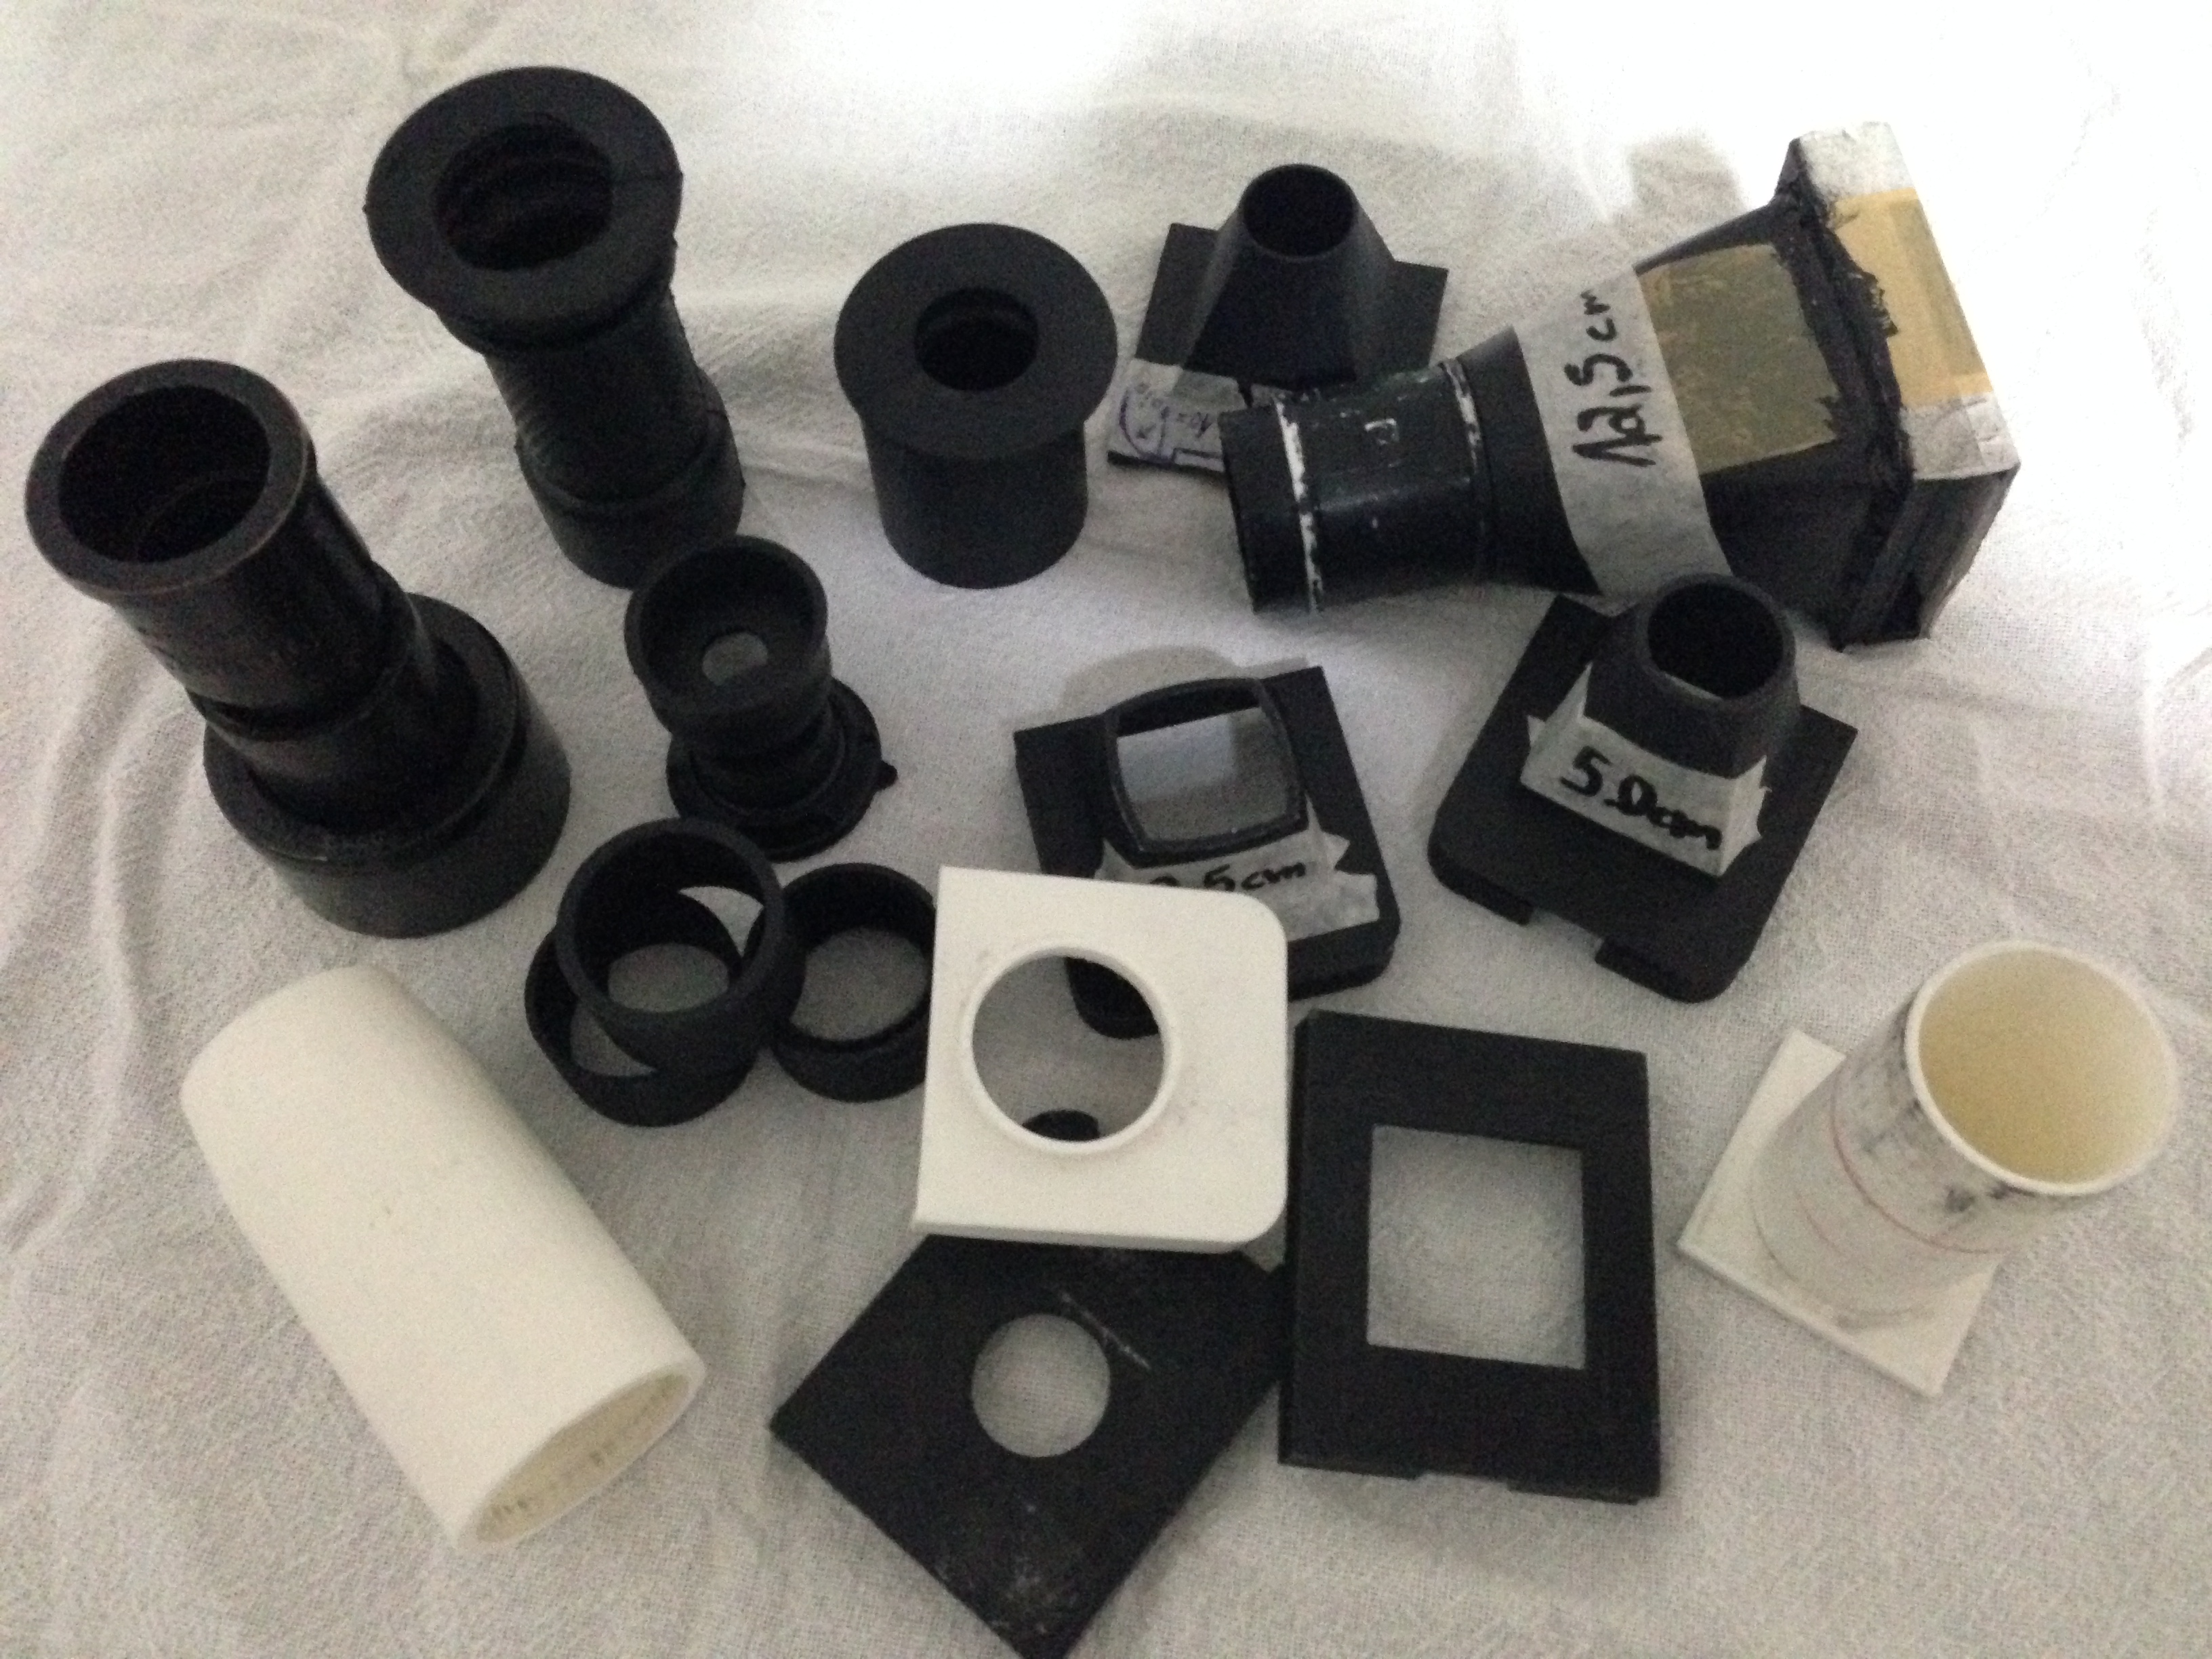
\includegraphics[height=0.45\linewidth]{__Images/05/52/older_versions.JPG}
		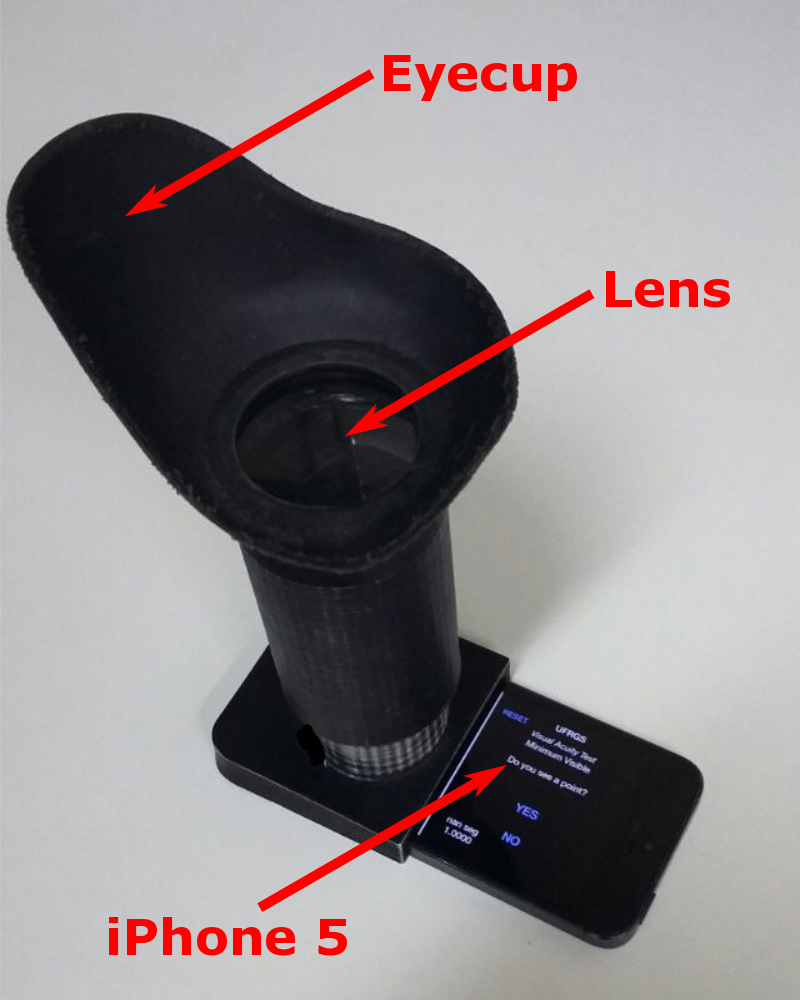
\includegraphics[height=0.45\linewidth]{__Images/05/52/newpic.png}
		\label{fig:prototype}
	}
	\subfigure[]{
		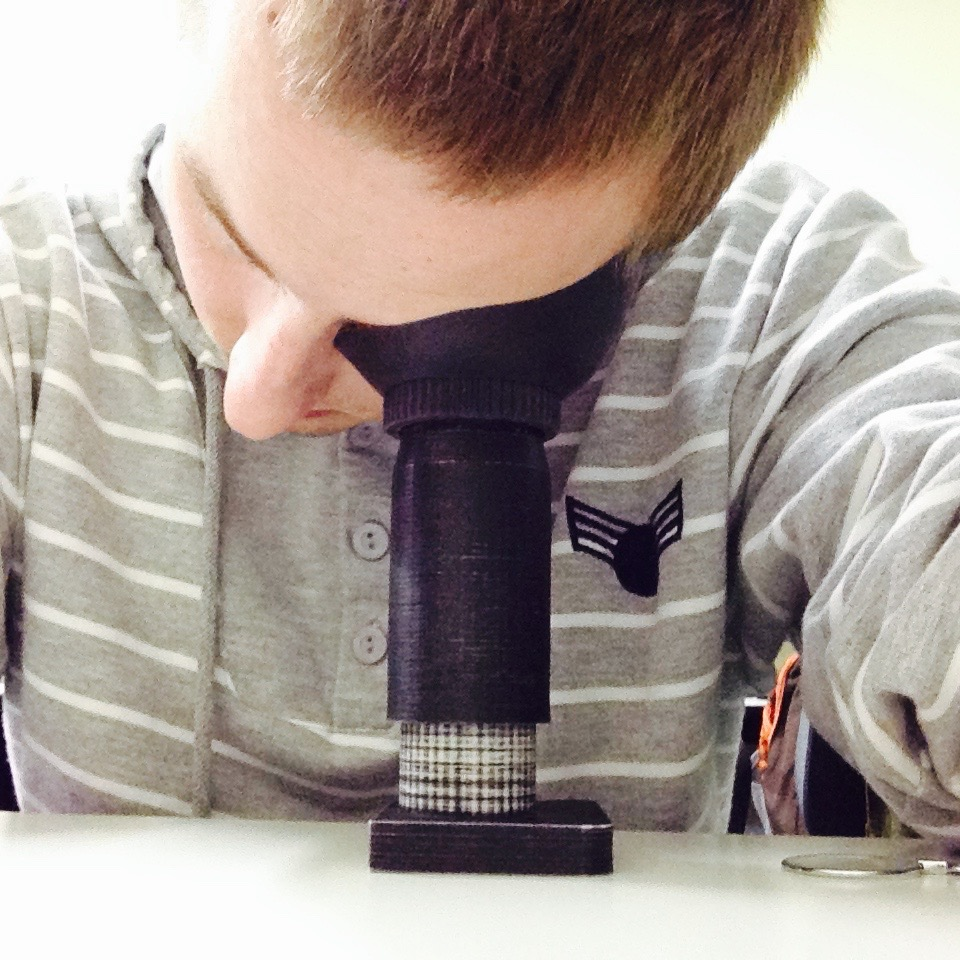
\includegraphics[height=0.45\linewidth]{__Images/05/52/frontview.jpg}
		\label{fig:Matheus_using_aparatus}
	}
	\caption[Estimating absolute threshold for vision]{Estimating absolute threshold for vision. (a) Apparatus designed for the psychophysical evaluations. It consists of a 12.5 cm long tube painted inside with dull black paint, with an 8.0 D plano-convex lens and an eyecup at one end, and an iPhone 5 at the other end. (b) A person during an evaluation.}
	\label{fig:3d_apparatus}
\end{figure}


To measure the amount of light emitted by the iPhone 5, we  used a digital light meter (Minipa, model MLM-1020) supported 3.0 cm above the smartphone's screen by a samll black cylinder (Figure \ref{fig:iPhone_luximeter}). The light meter (luximeter) and the iPhone were connected to a MacBook Pro laptop through USB connections. A program in the laptop controlled the intensity of a single pixel displayed in the central region of the iPhone screen and read the measurement made by the luximeter (Figure \ref{fig:pc_iPhone_luximeter}). The intensity values ranged from 0.0 to 1.0 in steps of 0.05 (a total of 21 measurements). The readings were made after the pixel with the desired intensity has been displayed for five seconds to allow the luximeter enough time to stabilize its reading. At the end of this procedure, we obtained a response curve relating all stimulus values to lux values. 
%Figure \ref{fig:luximeter} illustrate the adaptation made to isolate external light and maintain the correct distance, the light meter, and the wood device used at the lab. This analysis allowed us to generate a surface relating lux values with the stimulus' size and intensity. 

\begin{figure}[!hbt]
	\centering
	\subfigure[]{
		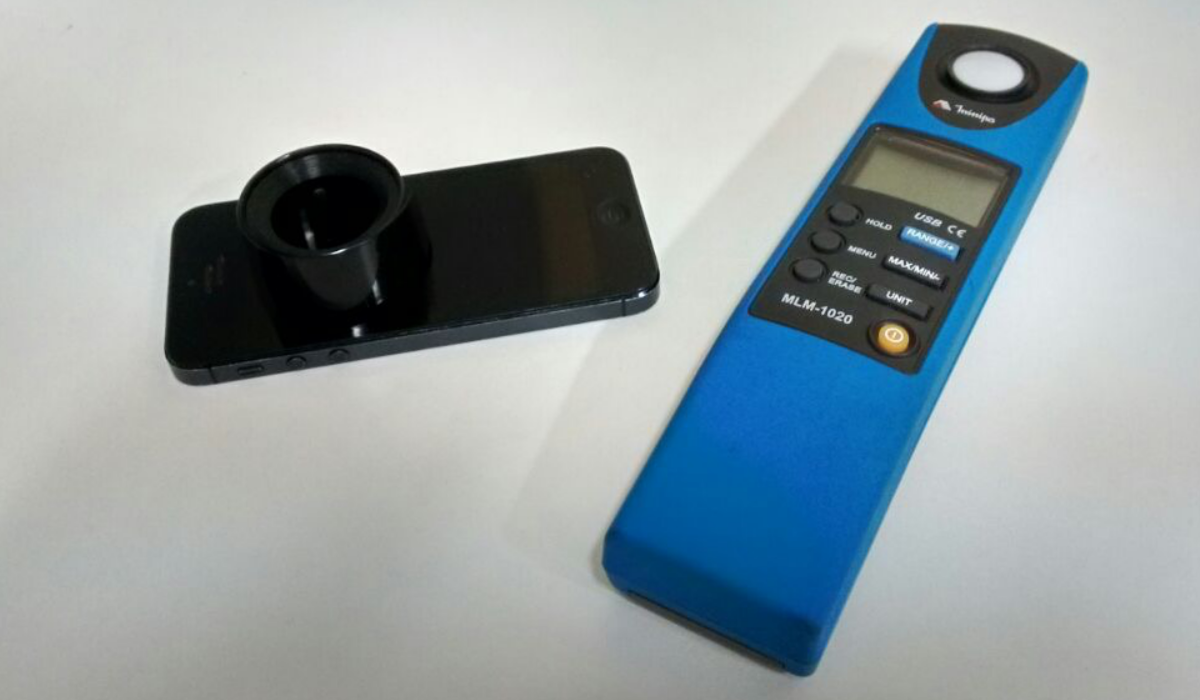
\includegraphics[width=0.45\linewidth]{__Images/05/52/cell+lux.png}
		\label{fig:iPhone_luximeter}
	}
	\subfigure[]{
		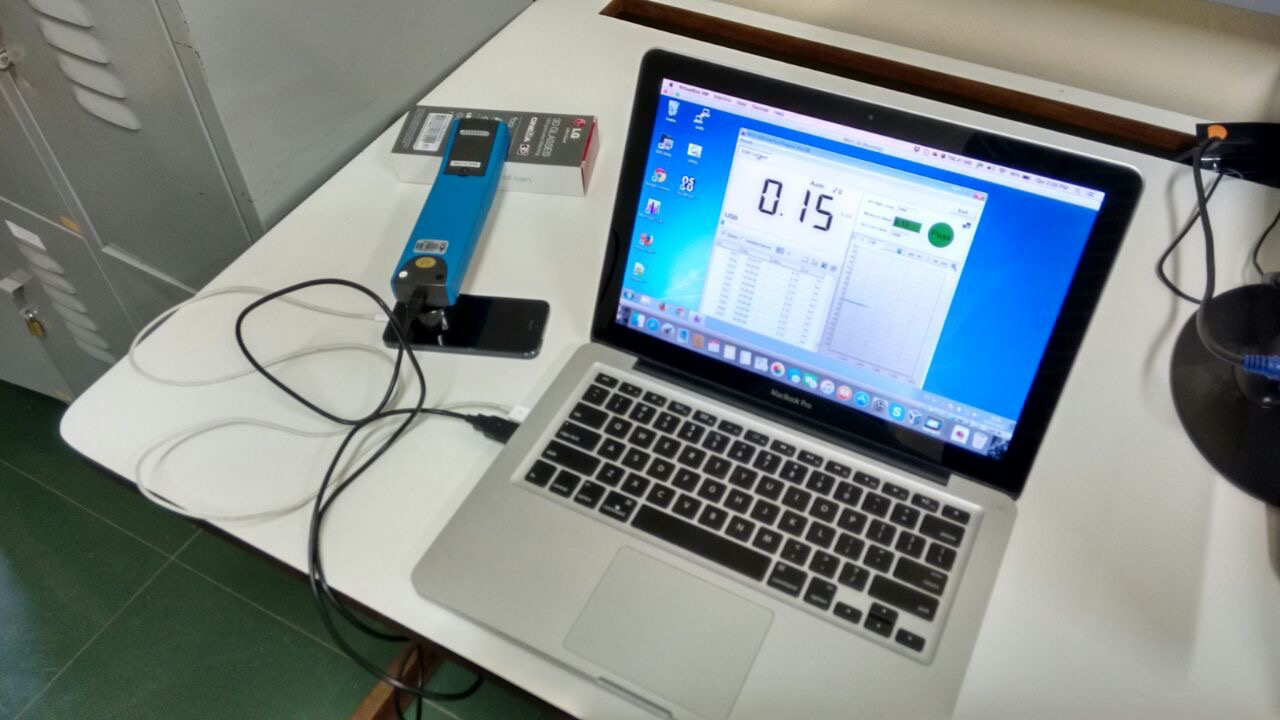
\includegraphics[width=0.45\linewidth]{__Images/05/52/pc_luximetro.jpg}
		\label{fig:pc_iPhone_luximeter}
	}
	
	\caption[Calibration procedure]{Calibration procedure. (a) A luximeter (Minipa, model MLM-1020) and the iPhone 5 the a 3.0 cm tall black cylinder used to hold the luximeter during the light measurements. (b) A MacBook Pro laptop controls the intensity values displayed on a single pixel and reads the values measured by the luximeter.  }
	\label{fig:luximeter}
\end{figure}
%\begin{figure}[!b]
	%\centering
	%
	%\subfigure[]{
%%		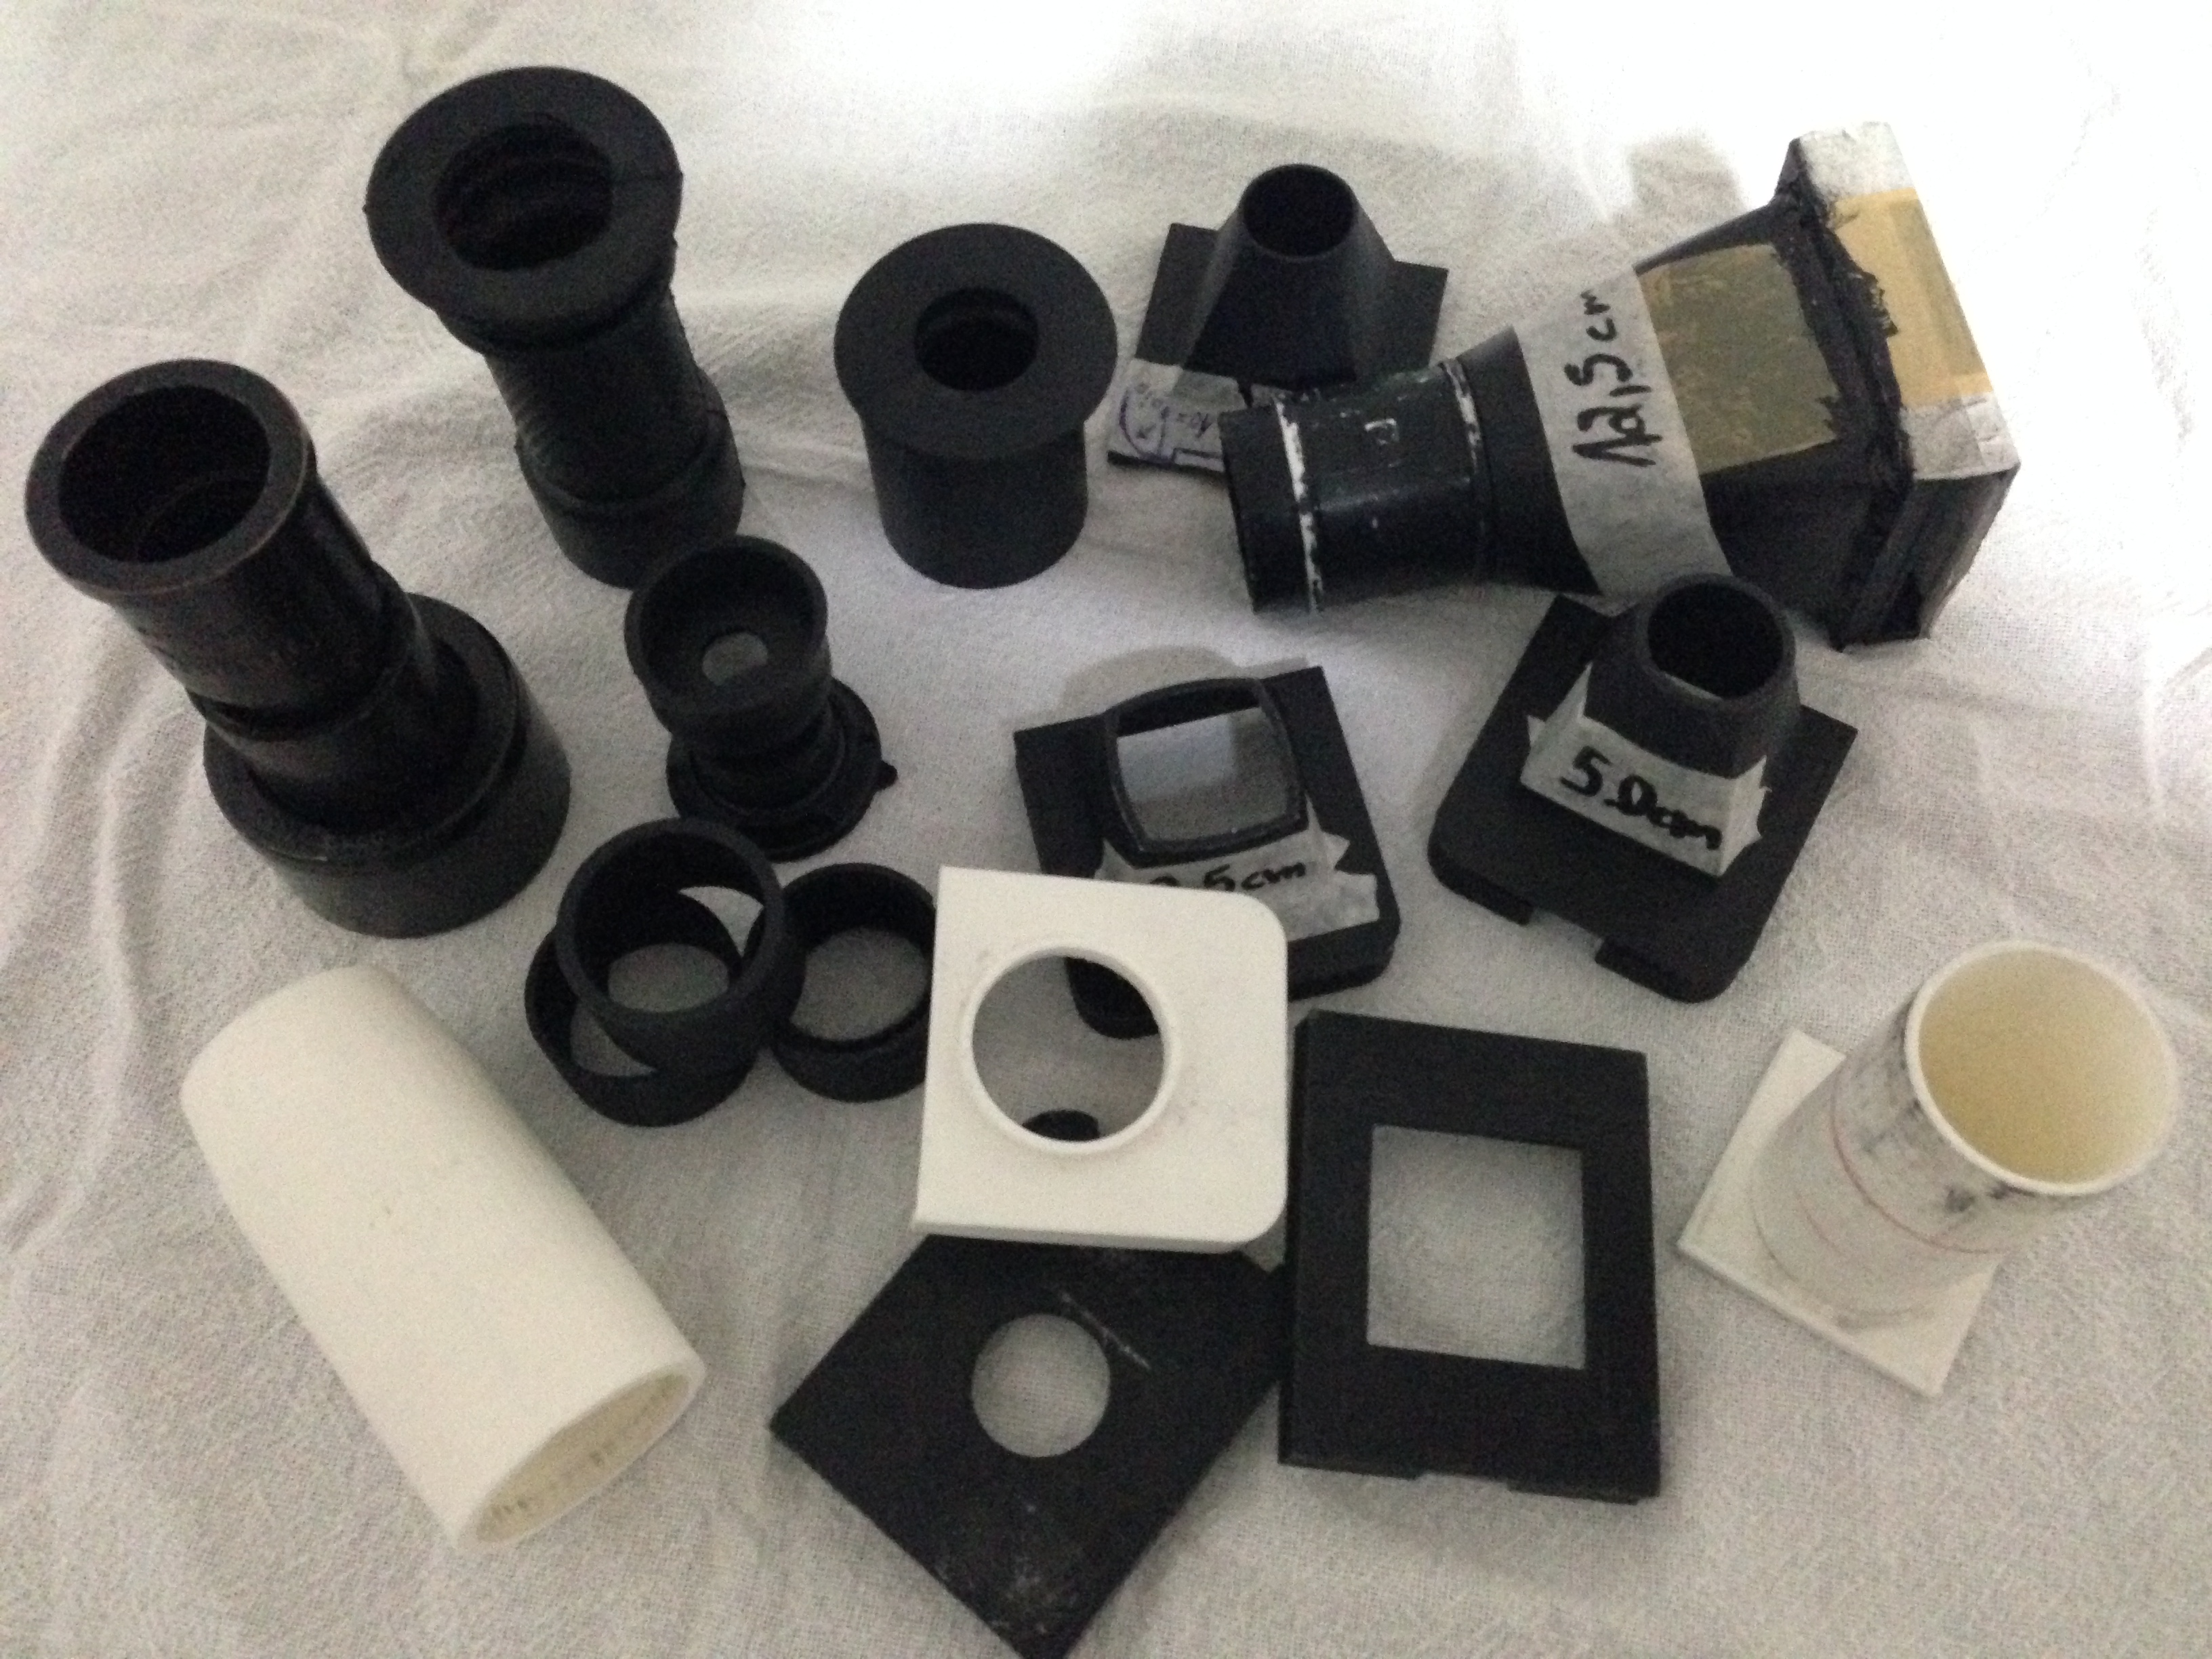
\includegraphics[height=0.45\linewidth]{__Images/05/52/older_versions.JPG}
		%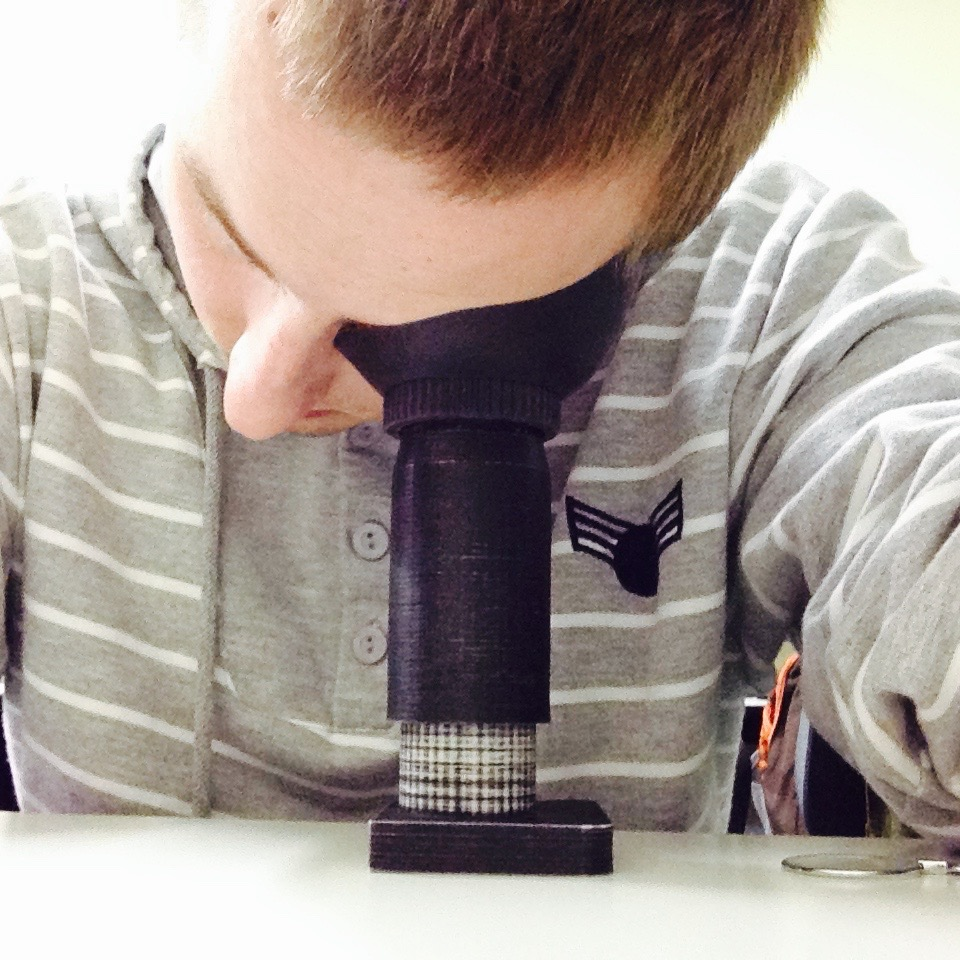
\includegraphics[height=0.45\linewidth]{__Images/05/52/frontview.jpg}
		%\label{fig:prototype}
	%}
	%~
	%\subfigure[]{
%%		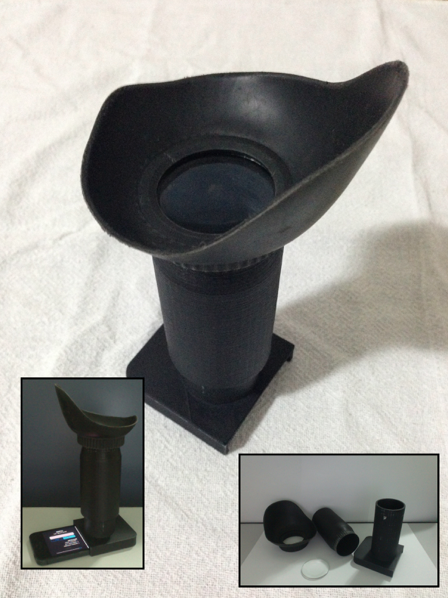
\includegraphics[height=0.45\linewidth]{__Images/05/52/new_version.png}
		%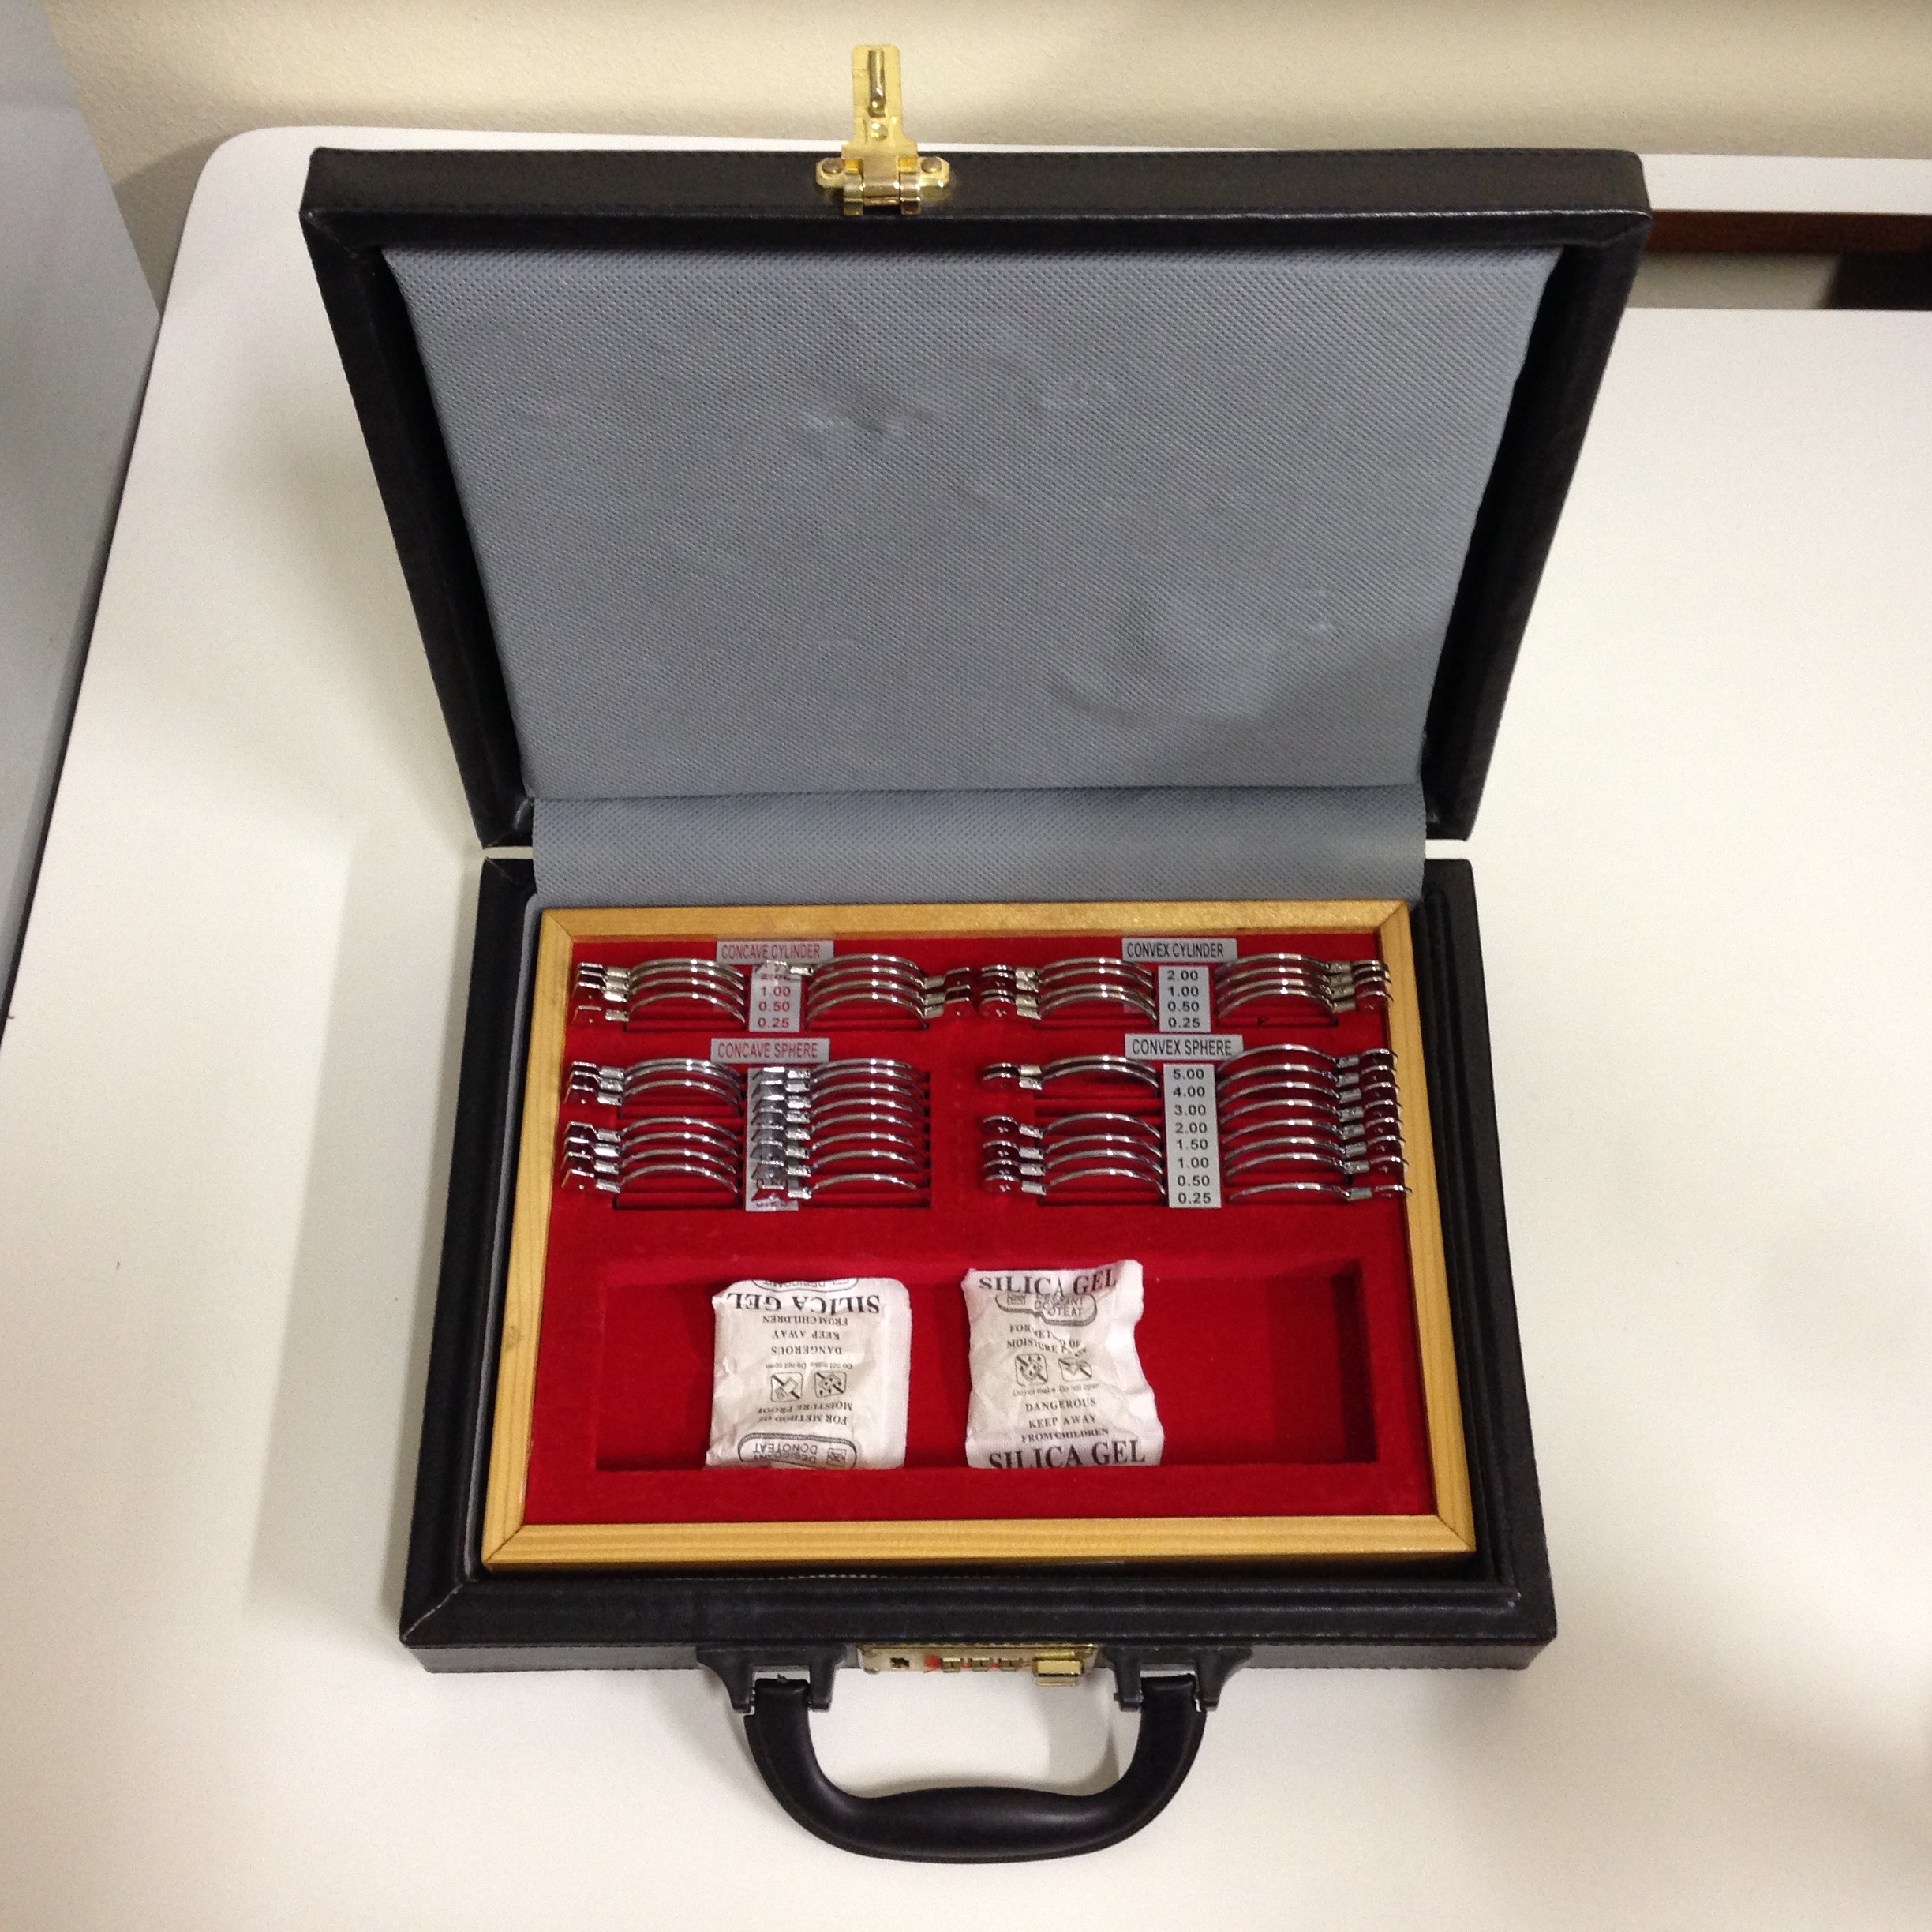
\includegraphics[height=0.45\linewidth]{__Images/05/52/lensset.jpg}
		%\label{fig:new_prot}
	%}
	%
	%\caption[XXX]{XXX}
	%\label{fig:XXX}
%\end{figure}



%Medical data from 20 subjects were captured with specialized ophthalmic equipment from a partner clinic. This data is fully described in Appendix \ref{chap:AppendixB}, together with the results of all absolute threshold psychophysical evaluations. We've realized absolute threshold experiments as described in \ref{subsec:ExperimentalDesign}, and selected two groups of them to present partial results --- from subject 1 (hyperopic) and 11 (myopic). 

\section{Results}

Figure~\ref{fig:hyperopic_myopic} presents plots summarizing the psychophysical experimental results for two subjects: a hyperopic (Figure~\ref{fig:myplot_1}) and a myopic (Figure~\ref{fig:myplot_11}). In these plots, the horizontal axis shows the power of the additional lenses used in the experiment (from -5.0 to +5.0 diopters). The numbers in vertical axis are the iPhone intensity values in the $[0,1]$ range.
%for each subject that combines the result of four psychophysical experiments. 
The blue lines shows the minimum intensity perceived by the individuals when using cycloplegic eyedrops. 
%the additional lenses from -5.0 to +5.0 diopters. 
%It also consider the use of eyedrops. 
The red ones are the mean of three psychophysical evaluations without the use of eyedrops (\ie, crystalline lens can and will accommodate more if necessary). The dashed lines show the data of the right eye, while solids correspond to the left eye. The circles show the overall minimum intensity value (\ie, considering the results of all lenses). The black lines indicate the individual's spherical equivalent refraction (SER).
%
\begin{figure}[!thb]
	\centering
	\subfigure[]{
		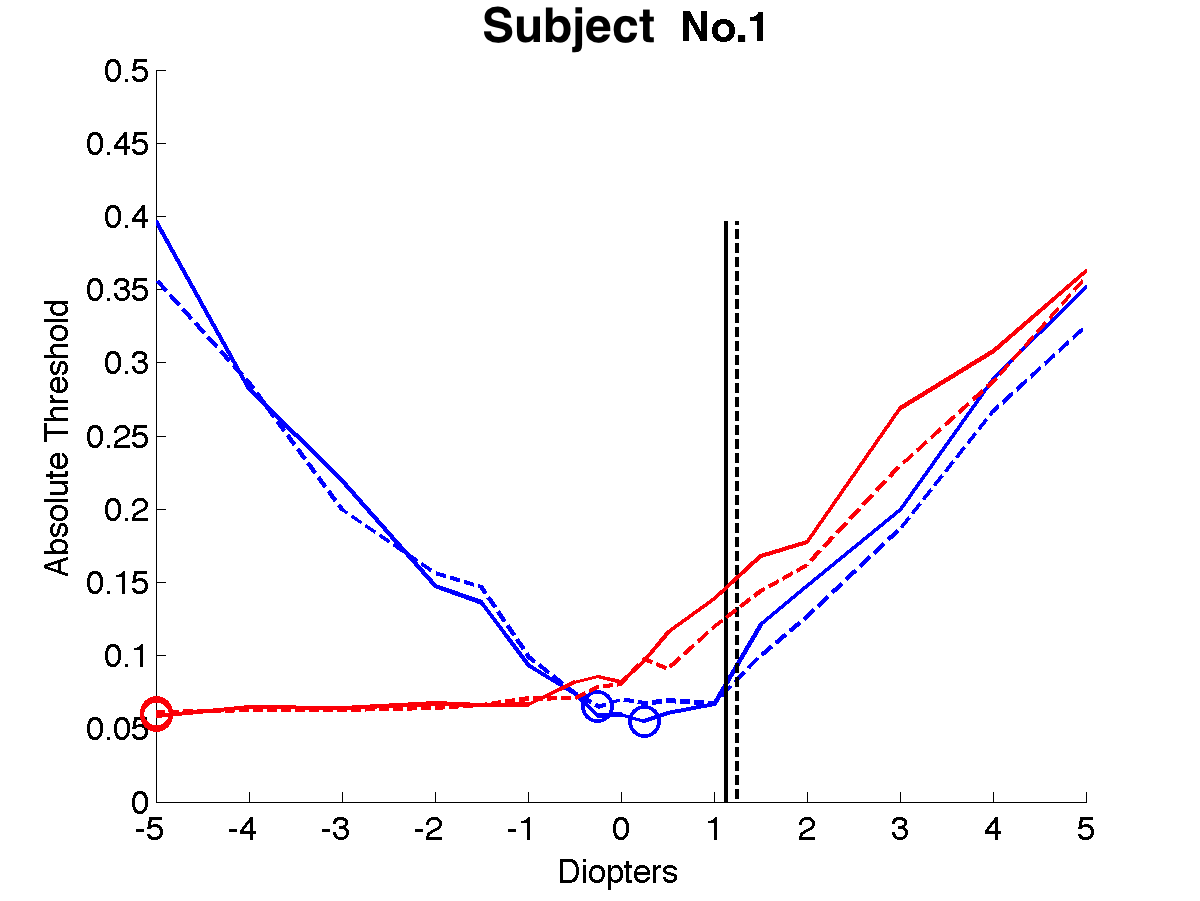
\includegraphics[width=0.47\linewidth]{__Images/05/52/myplot_1.png}
		\label{fig:myplot_1}
	}
	~
	\subfigure[]{
		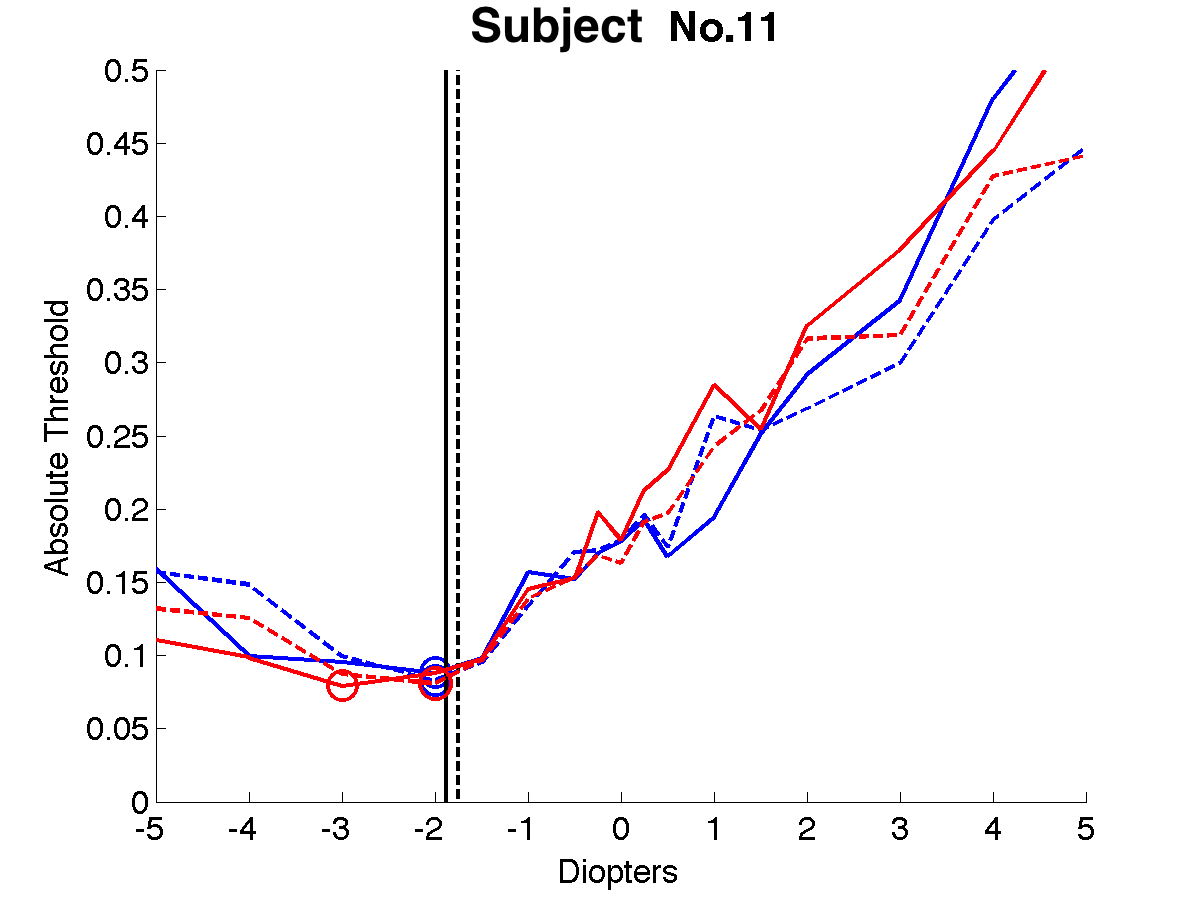
\includegraphics[width=0.47\linewidth]{__Images/05/52/myplot_11.png}
		\label{fig:myplot_11}
	}
	\caption[Plot of minimum intensity perceived with and without cycloplegic eyedrops for two sub- jects from the sample]{Plot of minimum intensity perceived with and without cycloplegic eyedrops for two subjects from the sample. (a) a hyperopic. (b) a myopic.  The horizontal axes show the power of the additional lenses used in the experiment. The numbers in vertical axis are the iPhone intensity values in the $[0,1]$ range. 
	Blue and red lines indicate results with and without cycloplegia, respectively. 
	The dashed lines show the data of the right eye, while solids correspond to the left eye. The circles show the overall minimum intensity values, and the black vertical lines show the spherical equivalent refraction values.}
	\label{fig:hyperopic_myopic}
\end{figure}

To better understand the impact of accommodation in the determination of the absolute threshold, we have performed a controlled experiment involving a single eye of one subject. This subject received three drops of the cycloplegic eyedrop, and performed the described psicophysical evaluation twice: fifteen minutes after receiving the last drop, and four hours later. The results of this experiment are illustrated in Figure~\ref{fig:variation_pics}. Figure~\ref{fig:pupil} shows the apparent effect --- mydriasis (\ie, the dilation of the pupil) in the tested eye. As can be seen in Figure~\ref{fig:AT-variation}, the evaluation performed fifteen minutes after the eyedrop administration (red line) shows a minimum intensity detected when the additional +1.0 D lens has been used. Note this is very close to the SER value of +1.25 D estimated by the autorefractor. In turn, four hours after (green line) the minimum intensity was detected with a -0.25 D lens. The evaluation performed before the cycloplegia (blue line) resulted in the minimum intensity detected for a -1.0 D lens.

%higher dosages and short time (red line) values almost correspond to the aberration captured by the gold standard ophthalmic equipment.
%Due to the cycloplegic concentration, this effect lasted for ten days. 

\begin{figure}[!t]
	\centering
	
	\subfigure[]{
		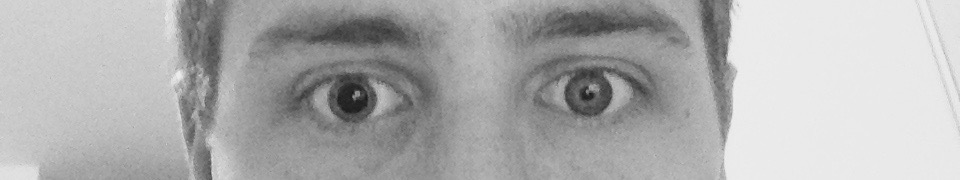
\includegraphics[width=1.00\linewidth]{__Images/05/52/pupil_matheus.jpg}
		\label{fig:pupil}
	}
	
	\subfigure[]{
		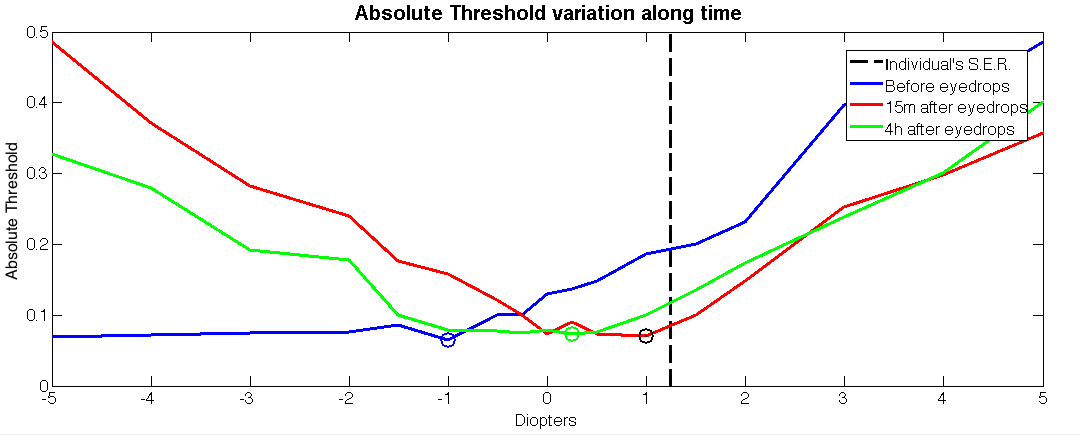
\includegraphics[width=1.00\linewidth]{__Images/05/52/newT_matheus_AT-variation.png}
		\label{fig:AT-variation}
	}
	
	\caption[Impact of accommodation in the detection of the minimum intensity]{Impact of accommodation in the detection of the minimum intensity. (a) Eye after administration of cycloplegic eyedrops. (b) Plot of the minimum-intensity detection before and after the use of cyclopegic eyedrops.  }
	\label{fig:variation_pics}
\end{figure}

According to our hypothesis, the minimum detected intensity should be perceived when the power of the additional lens approaches the subject's SER, since this would reduce the size of the circle of confusion. In practice, one's tendency to accommodate tends to shift the minimum detected value to the left (requiring more negative power to compensate for the accommodation). 
The tendency of patients to accommodate and ask for more negative power during eye examination is a well-known fact among ophthalmologists~\cite{Kronbauer2015}. 
As a result, we have observed that a single drop of cycloplegic drug brings the measured result closer to the expected one (according to our hypothesis) when compared to evaluations performed without the use of eyedrops. However, the use of a single drop can only partially avoid accommodation. As such, the result observed with the use of three drops were considerably closer to the expected one than when the evaluation was performed with a single drop. This conclusion can be observed in Figures~\ref{fig:pop_1} and \ref{fig:pop_11}, which show a more detailed analysis of the results obtained for both eyes of the hyperopic and myopic subjects in Figure~\ref{fig:hyperopic_myopic}, with and without eye partial cycloplegia (\ie, with one drop, and with no drops).  

%Considering that absolute threshold values tends to increase according to the lens power, and 
To perform this analysis, we have used a least-squares fitting technique to obtain a second-order polynomial representation of the minimum intensity detected by these individuals. We have also computed the correlation-coefficient matrix and evaluated the fitting parameters to calculate confidence intervals for the responses. Such intervals (confidence bounds) are illustrated by red-dashed lines in Figures~\ref{fig:pop_1} and \ref{fig:pop_11}. The green lines are the minimum detected intensity values obtained in the psychophysical evaluations with (Figures~\ref{fig:pop_1-1} and \ref{fig:pop_11-1}) and without (Figures~\ref{fig:pop_1-0} and \ref{fig:pop_11-0}) the use of eyedrops. The best-fitting curve is shown in blue, and its minimum value is represented by a small blue circle.

\begin{figure}[!b]
	\centering
	
	\subfigure[with eye drops]{
		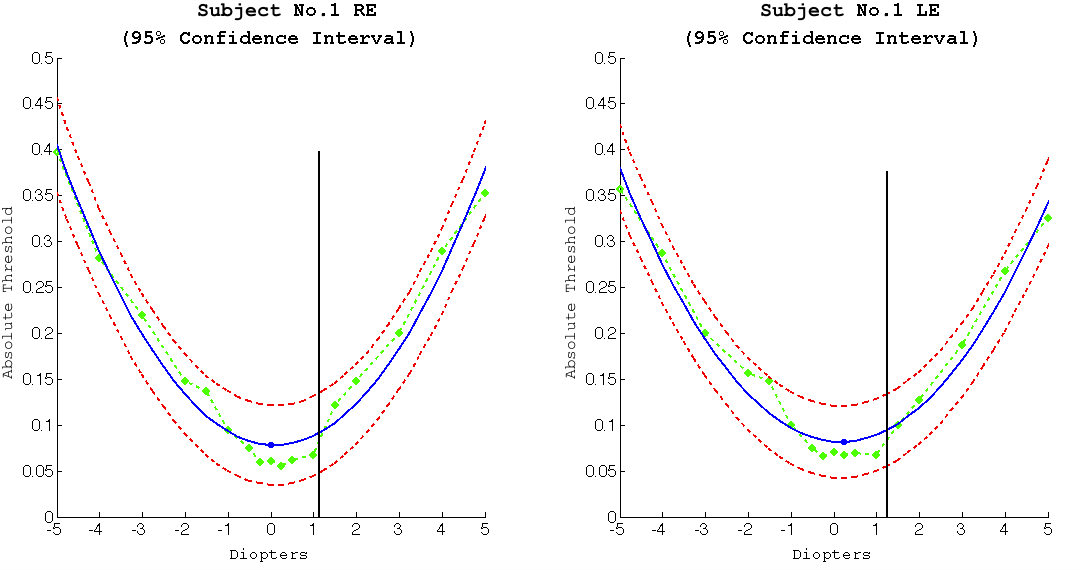
\includegraphics[width=1.00\linewidth]{__Images/05/52/pop_1-1(with_eyedrops).png}
		\label{fig:pop_1-1}
	}
	
	\subfigure[without eye drops]{
		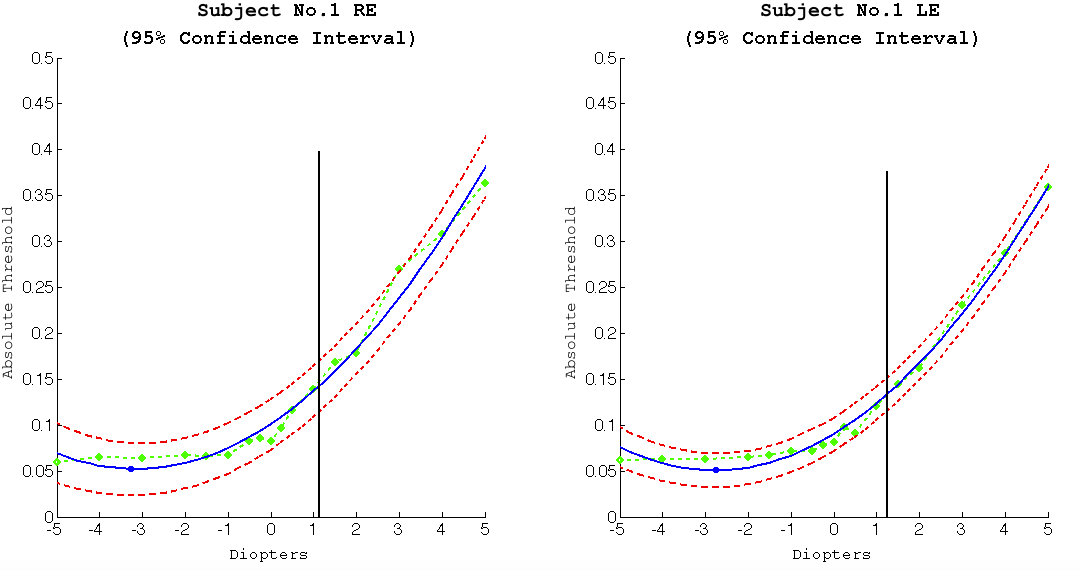
\includegraphics[width=1.00\linewidth]{__Images/05/52/pop_1-0(without_eyedrops).png}
		\label{fig:pop_1-0}
	}
	
	\caption[Polynomial fitting of the absolute threshold values of Subject 1]{Polynomial fitting (blue line) of the minimum intensity values for a hyperopic individual (Subject 1). The red lines define the confidence interval of 95\%. Each green point is the minimum value for a specific extra lens power. The minimum detected intensity is highlighted as a small blue circle. The black vertical line is the SER.}
	\label{fig:pop_1}
\end{figure}

\begin{figure}[!t]
	\centering
	
	\subfigure[with eye drops]{
		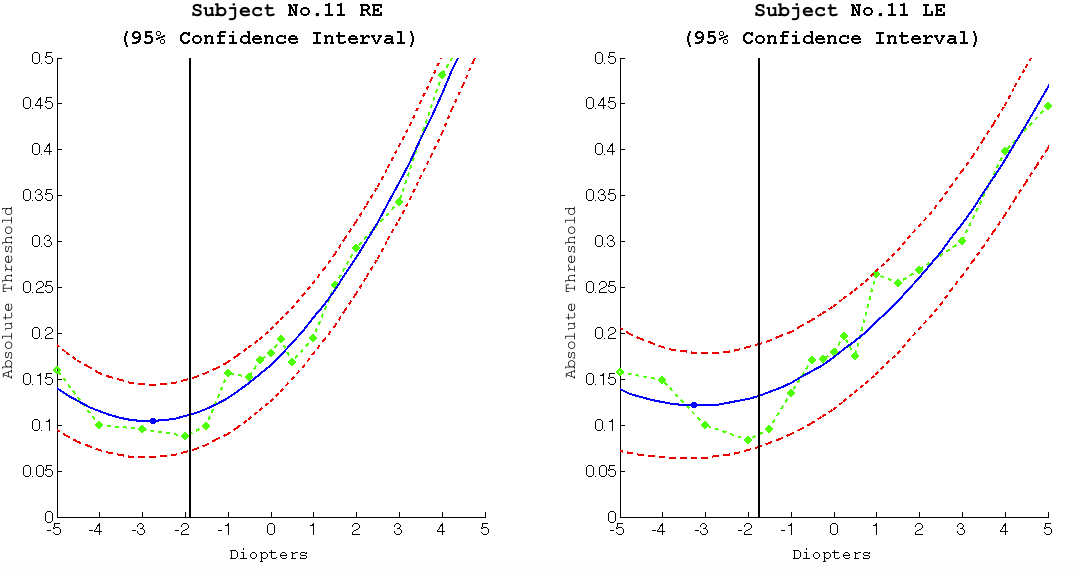
\includegraphics[width=1.00\linewidth]{__Images/05/52/pop_11-1(with_eyedrops).png}
		\label{fig:pop_11-1}
	}
	
	\subfigure[without eye drops]{
		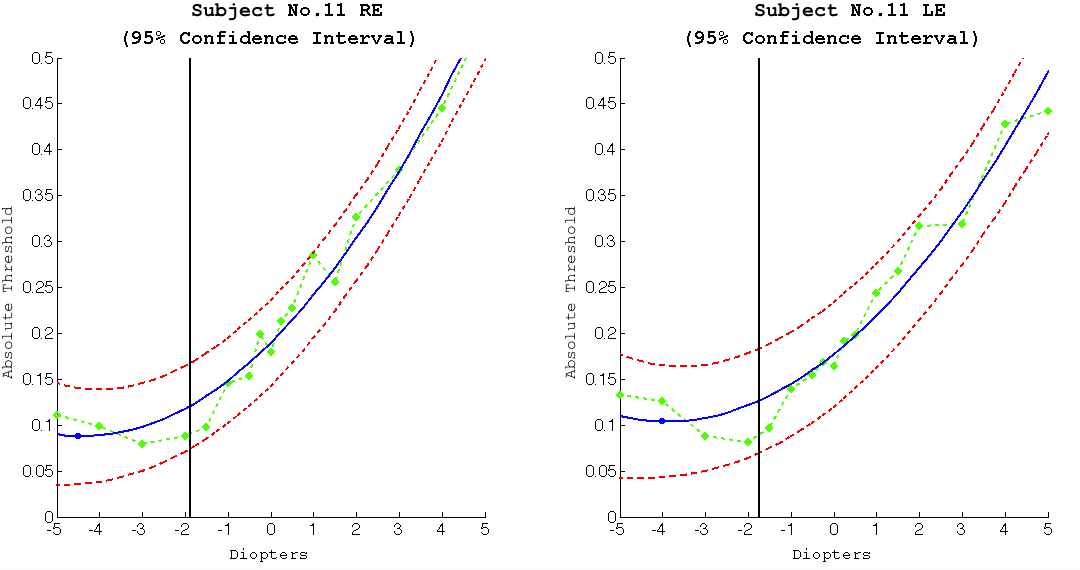
\includegraphics[width=1.00\linewidth]{__Images/05/52/pop_11-0(without_eyedrops).png}
		\label{fig:pop_11-0}
	}
	
	\caption[Polynomial fitting of the absolute threshold values of Subject 11]{Polynomial fitting (blue line) of the minimum intensity values for a myopic individual (Subject 11). The red lines define the confidence interval of 95\%. Each green point is the minimum value for a specific extra lens power. The minimum detected intensity is highlighted as a small blue circle. The black vertical line is the SER.}
	\label{fig:pop_11}
\end{figure}

When we formulated our hypothesis, we were looking for a simple, inexpensive, and non-invasive way of estimating one's spherical equivalent refraction based only on his/her absolute threshold for vision. 
Although we have not fully demonstrated our hypothesis, the graphs shown in Figures~\ref{fig:AT-variation}, \ref{fig:pop_1}, and \ref{fig:pop_11} provide strong evidence to support it. Although we believe that this hypothesis could be verified with higher doses of cycloplegic eyedrops, such an alternative is neither attractive or practical as a vision test. The administration of higher doses of cycloplegic drugs have undesirable side effects, which may last for weeks.  
 
\section{Summary}

This chapter described an attempt to estimate one's SER based on a measurement of his/her absolute threshold for vision. It presented our hypothesis to support such claim, and detailed a series of experiments and a device designed to verify such hypothesis. While we have obtained some evidence that supports its correction, the method turned out not to be a practical solution.
